\setchapterimage[6.5cm]{seaside}
\setchapterpreamble[u]{\margintoc}
\chapter[Figures and Tables]{Figures and Tables\footnotemark[0]}

\footnotetext{The credits for the image above the chapter title go to:
	Bushra Feroz --- Own work, CC~BY-SA~4.0, 
	\url{https://commons.wikimedia.org/w/index.php?curid=68724647}}

\section{Normal figures and tables}

可以像插入任何标准\LaTeX\xspace 文档一样插入数字和表。\Package{graphicx}包已经加载并配置好了,其图形宽度等于textwidth,并且调整了高度以保持原始的纵横比。正如您所想象的,标题将被很好地放置在页边空白处。这是在\Package{floatrow}包的帮助下实现的。

这里有一张蒙娜丽莎的照片(\reffig{normalmonalisa})作为例子。标题格式为页边距和边注;如果您想更改标题的某些内容,可以使用\Package{title}包中的命令\ command {captsetup}。请记住,如果您想引用一个图形,标签必须在标题\emph{之后}出现!

\begin{figure}[hb]
	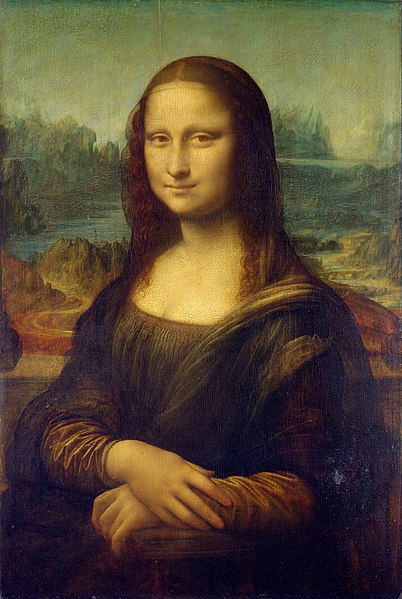
\includegraphics[width=0.45\textwidth]{monalisa}
	\caption[Mona Lisa, again]{It's Mona Lisa again. \blindtext}
	\labfig{normalmonalisa}
\end{figure}

虽然标题的格式由\Package{title}管理,但是它的位置由\Package{floatrow}包处理。取得这样的成绩是很辛苦的,但现在我很满意。在双面模式下,标题以正确的页边距打印。

插入表格和插入数字一样容易,如下面的代码所示:

\begin{lstlisting}
\begin{table}
\begin{tabular}{ c c c c }
	\toprule
	col1 & col2 & col3 & col 4 \\
	\midrule
	\multirow{3}{4em}{Multiple row} & cell2 & cell3 & cell4\\ &
	cell5 & cell6 & cell7 \\ &
	cell8 & cell9 & cell10 \\
	\multirow{3}{4em}{Multiple row} & cell2 & cell3 & cell4 \\ &
	cell5 & cell6 & cell7 \\ &
	cell8 & cell9 & cell10 \\
	\bottomrule
\end{tabular}
\end{table}
\end{lstlisting}

which results in the useless \vreftab{useless}.

\begin{table}[h]
\caption[A useless table]{A useless table.}
\labtab{useless}
\begin{tabular}{ c c c c }
	\toprule
	col1 & col2 & col3 & col 4 \\
	\midrule
	\multirow{3}{4em}{Multiple row} & cell2 & cell3 & cell4\\ &
	cell5 & cell6 & cell7 \\ &
	cell8 & cell9 & cell10 \\
	\multirow{3}{4em}{Multiple row} & cell2 & cell3 & cell4 \\ &
	cell5 & cell6 & cell7 \\ &
	cell8 & cell9 & cell10 \\
	\bottomrule
\end{tabular}
\end{table}

I don't have much else to say, so I will just insert some blind text. 
\blindtext

\section{Margin figures and tables}

可以使用\Environment {marginfigure}环境插入Marginfigures。在这种情况下,整个图片被限制在页边空白处,标题在它下面。\reffig{marginmonalisa}是这样得到的:

\begin{lstlisting}
\begin{marginfigure}
	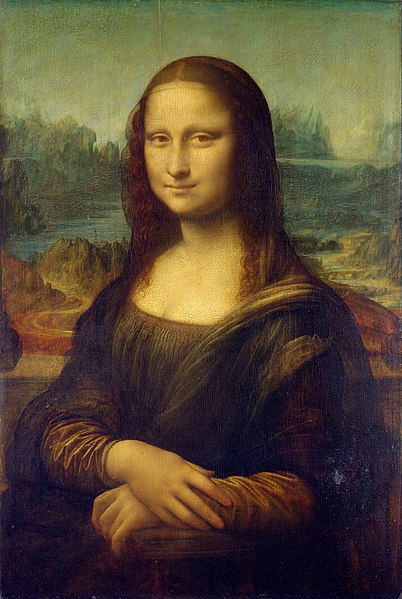
\includegraphics{monalisa}
	\caption[The Mona Lisa]{The Mona Lisa.}
	\labfig{marginmonalisa}
\end{marginfigure}
\end{lstlisting}

There is also the \Environment{margintable} environment, of which 
\reftab{anotheruseless} is an example. Notice how you can place the 
caption above the table by just placing the \Command{caption} command 
before beginning the \Environment{tabular} environment. Usually, figure 
captions are below, while table captions are above. This rule is also 
respected for normal figures and tables: the captions are always on the 
side, but for figure they are aligned to the bottom, while for tables to 
the top.

\begin{margintable}
\caption[Another useless table]{Another useless table.}
\labtab{anotheruseless}
\raggedright
\begin{tabular}{ c c c c }
	\hline
	col1 & col2 & col3 \\
	\hline
	\multirow{3}{4em}{Multiple row} & cell2 & cell3 \\ & cell5 & cell6 
	\\ & cell8 & cell9 \\ \hline
\end{tabular}
\end{margintable}

Marginfigures and tables can be positioned with an optional offset 
command, like so:

\begin{lstlisting}
\begin{marginfigure}[offset]
	\includegraphics{images/seaside}
\end{marginfigure}
\end{lstlisting}

Offset ca be either a measure or a multiple of \Command{baselineskip}, 
much like with \Command{sidenote}, \Command{marginnote} and 
\Command{margintoc}.\todo{Improve this part.} If you are wondering how I 
inserted this orange bubble, have a look at the \Package{todo} package.

\section{Wide figures and tables}

\begin{figure*}[h!]
	\includegraphics{seaside}
	\caption[一个宽阔的海边]{宽阔的海边,宽阔的标题。作品简介:布什拉·费罗兹(Bushra Feroz)著 --- 自己的工作, CC BY-SA 4.0, 
		\url{https://commons.wikimedia.org/w/index.php?curid=68724647}}
\end{figure*}

使用\Environment{figure*}和\Environment{table*}环境,您可以插入跨越整个页面宽度的数字。标题将根据口味被置于下方或上方。

您可能已经注意到了本章开头的全宽图像:但是,它是以一种完全不同的方式设置的,您将在\vrefch{layout}中了解到这一点。现在是处理超引用的时候了。
